
% \documentclass[manuscript]{aastex}
\documentclass[12pt,preprint]{aastex}
%\documentclass[preprint2]{aastex}
%\documentclass[aaspp4]{aastex}
%\documentclass{aastex}
%\documentclass[]{emulateapj}
%\documentclass[onecolumn]{emulateapj}

%!TEX TS-program=latex
\usepackage{amsmath}
%\usepackage{pdfsync}
%\def\snp{SN\,II-P} 
%\def\snep{SNe\,II-P} 
%\def\VmI{\hbox{$V\!-\!I$}} 
%\def\fe{\ion{Fe}{2}}
%\newcommand{\bvri}{\protect\hbox{$BV\!RI$} }

\citestyle{aa}

\begin{document}

% \slugcomment{Draft \today}
%\submitted{Draft \today} 

\title {Ay 190 Worksheet 2} 
\shorttitle{WS2}
\shortauthors{Kleiser}

\author{Io Kleiser} \affil{Caltech} \email{ikleiser@caltech.edu}

\section{Integration via Newton-Cotes Formulae}
This problem calls for the integration of (a) $\sin x$ and (b) $x \sin x$ over the interval $[0,\pi]$ using both trapezoidal and Simpson's methods. The values of the integration are shown in Figures \ref{f:trapsimp_sinx} and \ref{f:trapsimp_xsinx} and are shown to converge to the correct values for small stepsize $h$.

\begin{figure}[!ht]
\begin{center}
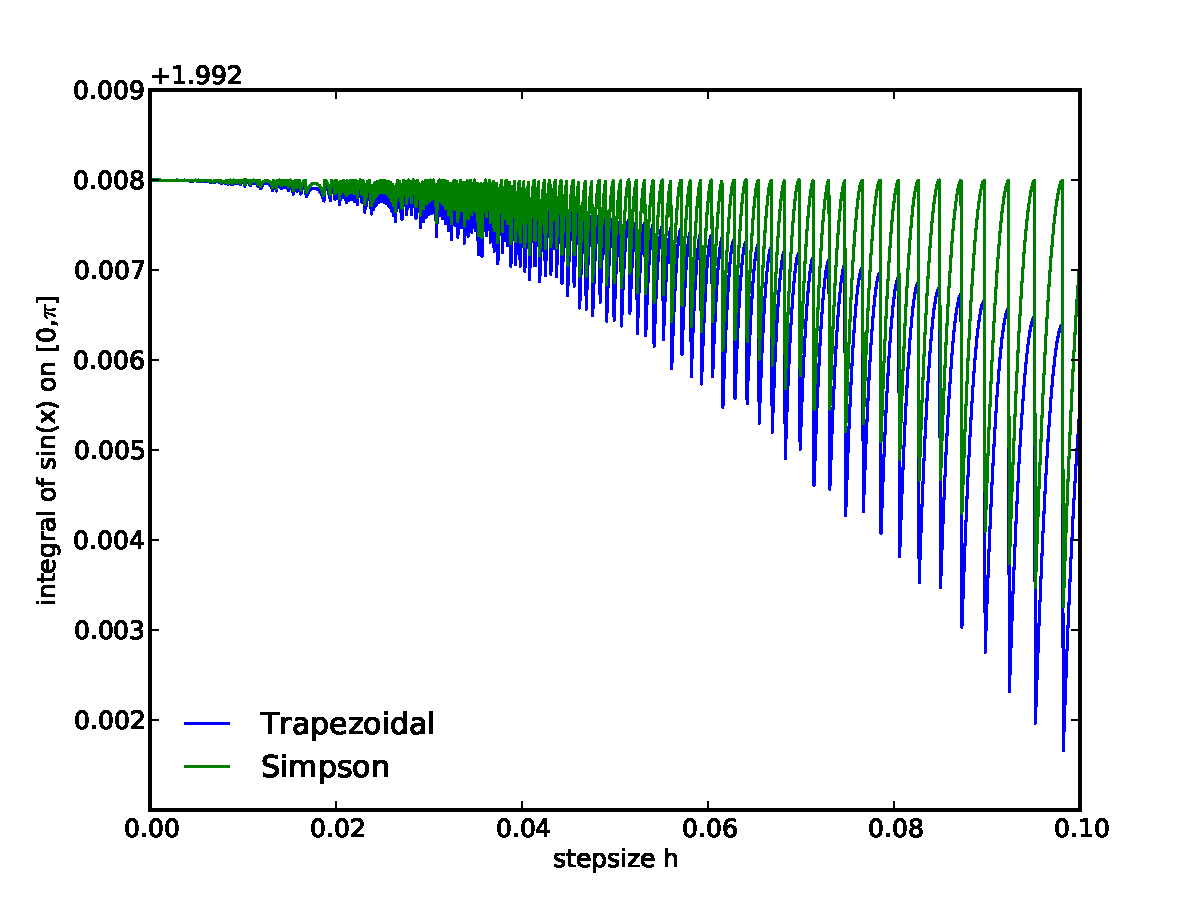
\includegraphics[width=6in]{trapsimp_sinx.pdf}
\end{center}
\caption{Integration of $\sin x$ via trapezoidal and Simpson's rule with varying stepsize $h$. \label{f:trapsimp_sinx}}
\end{figure}

\begin{figure}[!ht]
\begin{center}
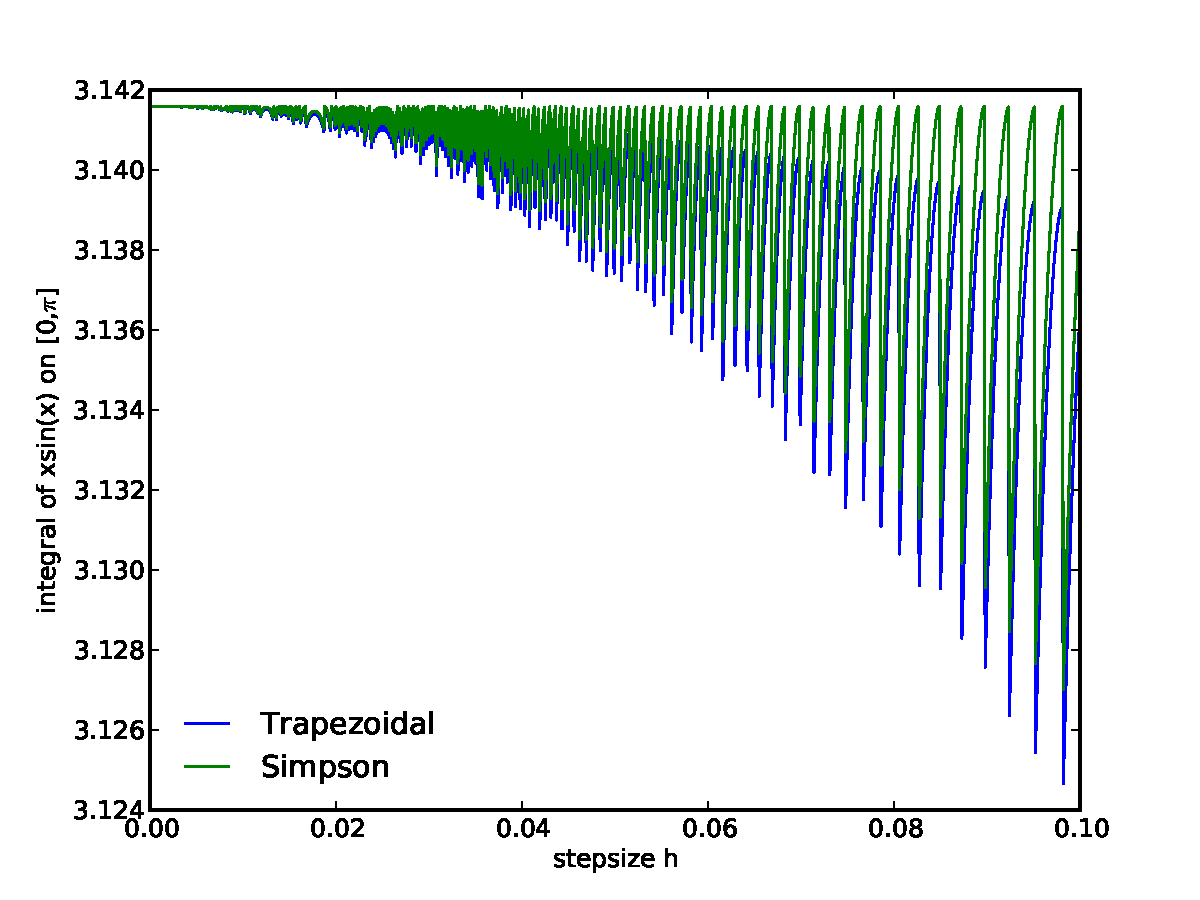
\includegraphics[width=6in]{trapsimp_xsinx.pdf}
\end{center}
\caption{Same as Fig. \ref{f:trapsimp_sinx} but for $x \sin x$. \label{f:trapsimp_xsinx}}
\end{figure}

%\bibliographystyle{apj2} 
%\bibliography{gal}

%\bibliography
\end{document}
